\documentclass{article}
\usepackage{tikz}
\usetikzlibrary{arrows,backgrounds,calc,trees}

\pgfdeclarelayer{background}
\pgfsetlayers{background,main}


\newcommand{\convexpath}[2]{
[   
    create hullnodes/.code={
        \global\edef\namelist{#1}
        \foreach [count=\counter] \nodename in \namelist {
            \global\edef\numberofnodes{\counter}
            \node at (\nodename) [draw=none,name=hullnode\counter] {};
        }
        \node at (hullnode\numberofnodes) [name=hullnode0,draw=none] {};
        \pgfmathtruncatemacro\lastnumber{\numberofnodes+1}
        \node at (hullnode1) [name=hullnode\lastnumber,draw=none] {};
    },
    create hullnodes
]
($(hullnode1)!#2!-90:(hullnode0)$)
\foreach [
    evaluate=\currentnode as \previousnode using \currentnode-1,
    evaluate=\currentnode as \nextnode using \currentnode+1
    ] \currentnode in {1,...,\numberofnodes} {
-- ($(hullnode\currentnode)!#2!-90:(hullnode\previousnode)$)
  let \p1 = ($(hullnode\currentnode)!#2!-90:(hullnode\previousnode) - (hullnode\currentnode)$),
    \n1 = {atan2(\x1,\y1)},
    \p2 = ($(hullnode\currentnode)!#2!90:(hullnode\nextnode) - (hullnode\currentnode)$),
    \n2 = {atan2(\x2,\y2)},
    \n{delta} = {-Mod(\n1-\n2,360)}
  in 
    {arc [start angle=\n1, delta angle=\n{delta}, radius=#2]}
}
-- cycle
}


\begin{document}
\thispagestyle{empty}

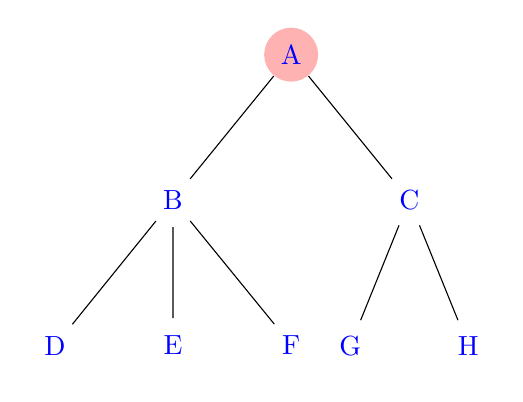
\begin{tikzpicture}
[
style0/.style={circle, draw=none, text centered, anchor=north, text=blue, text opacity=1},
style1/.style={circle, draw, fill=red,text centered, anchor=north, text=black, text opacity=1},
style2/.style={circle, draw, fill=red,fill opacity=0.3, text centered, anchor=north, text=black, text opacity=1, radius=3cm},
style3/.style={circle, draw=none, fill=blue,fill opacity=0.3, text centered, anchor=north, text=black, text opacity=1},
style4/.style={circle, draw=none, fill=green,fill opacity=0.3, text centered, anchor=north, text=black, text opacity=1},
	level distance=1.5cm,
  level 1/.style={sibling distance=3cm},
  level 2/.style={sibling distance=1.5cm}
  ]
\node  (A) [style2,style0] {A}
    child { node (B) [style0] {B} 
      child { node (D) [style0] {D}
    }
      child { node (E) [style0] {E}
    }
child { node (F) [style0] {F}
    }
  }
    child { node (C) [style0] {C}
      child { node (G) [style0] {G}
    }
child { node (H) [style0] {H}
    }
  };
\begin{pgfonlayer}{background}
%\fill[red,opacity=0.3] \convexpath{D,B,A,C,H,G,F,E}{10pt};
%\fill[blue,opacity=0.3] \convexpath{G,C,H}{10pt};
\end{pgfonlayer}
\end{tikzpicture}

\end{document}
